\section{Versuchsaufbau und Versuchdurchführung}

\begin{flushleft}
    Für den ganzen Versuch werden folgende Materialien benötigt:\\
    ein Labornetzgerät, zwei Kabel, zwei Isolatoren, ein Usb-Stick, ein \enquote{Temperatur Array}, eine Stoppuhr, 
    ein Datenlogger und eine Platte.\\
    \vspace{0.5cm}
    Auf der Platte, gezeigt in Abbildung \ref{Abbildung2}, sind vier Stäbe (Messing(schmal), Messing(breit), Aluminium, Edelstahl(V2A)), welche jeweils zwei Thermoelemente haben.
    In der Mitte dieser vier Stäben ist ein Peltierelement.
    Oben links befindet sich der Anschluss für das \enquote{Temperatur Array}. 
    Oben rechts befindet sich die Anschlüsse für das Labornetzgerät und ein Schalter, der auf "heat" oder "cool" gestellt werden kann.  
\end{flushleft}

\begin{figure}[H]
    \centering
    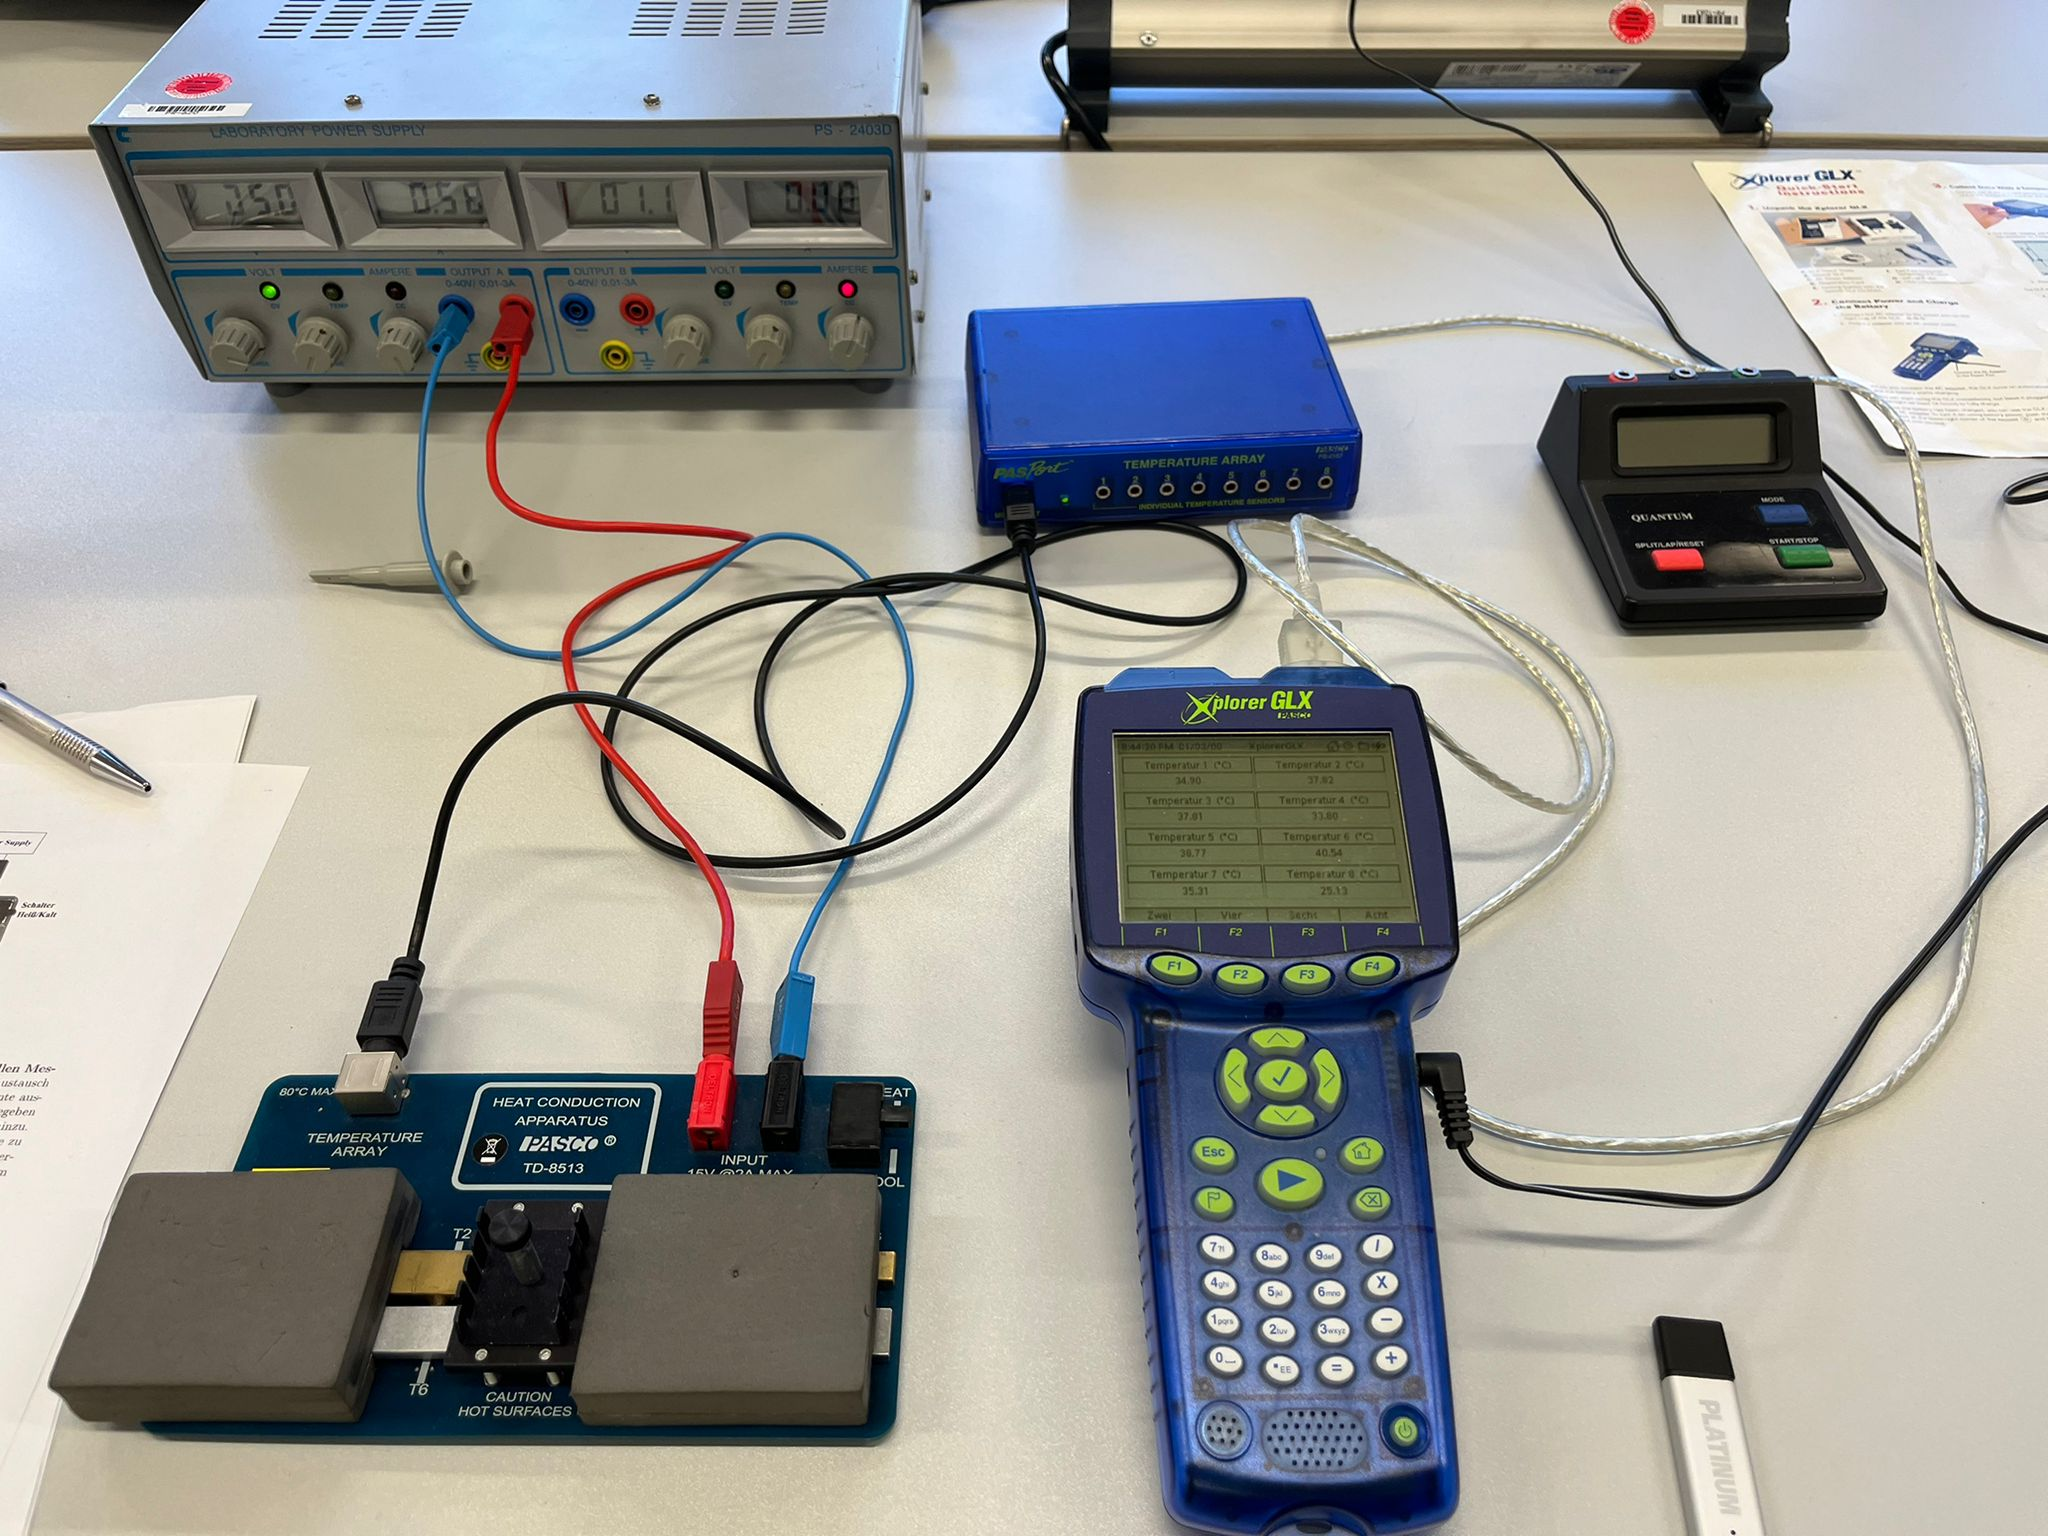
\includegraphics[height=80mm]{bilder/aufbau.jpeg}
    \caption{Die Abbildung der ganzen Versuchsmaterialien aufgebaut. \label{Abbildung1} }
\end{figure}

\begin{figure}[H]
    \centering
    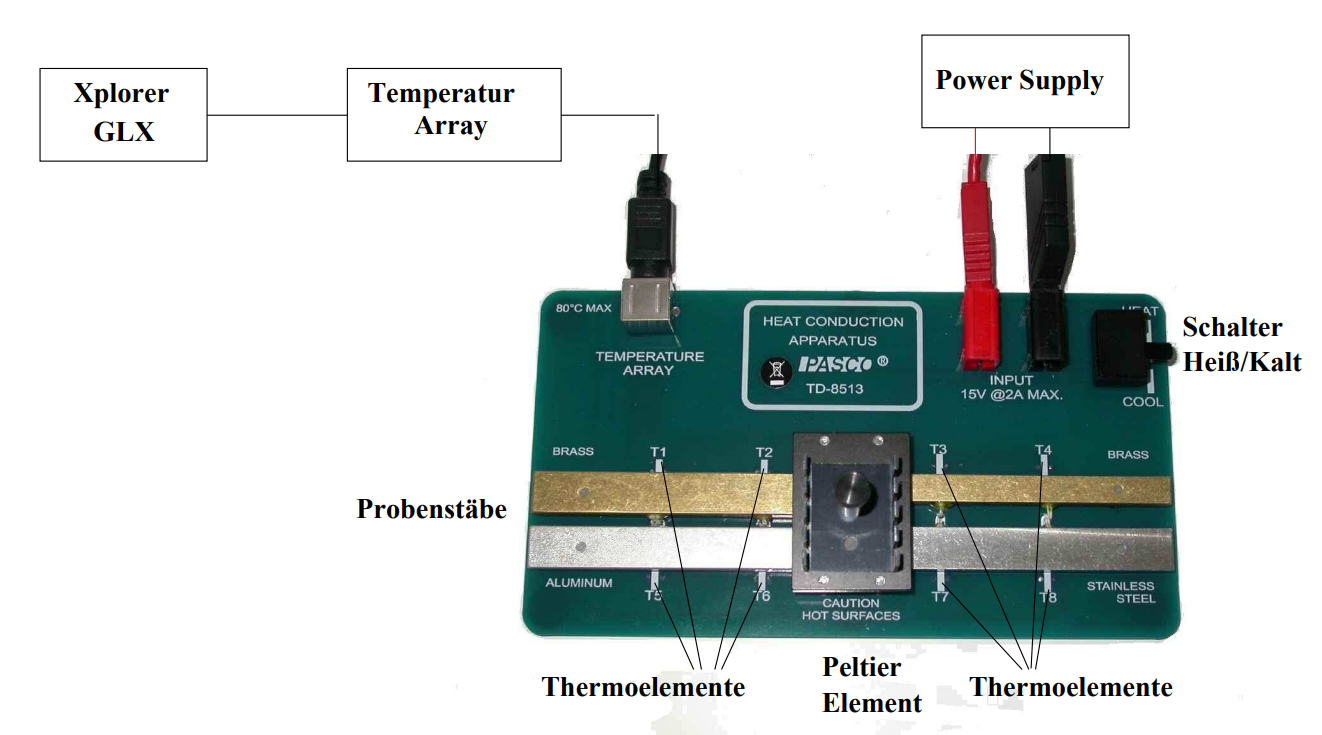
\includegraphics[height=80mm]{bilder/Platte1.png} 
    \caption{Eine Abbildung der Platte die in dem Versuch verwendet wird. \cite[3]{a1} \label{Abbildung2} }
\end{figure}


\begin{flushleft}
    Der Aufbau sieht wie folgt aus:\\
    Das eine Kabelende wird an das Labornetzgerät und das andere an die Platte angeschlossen. 
    Das Temperature Array wird mit der Platte verbunden und das \enquote{Temperatur Array} mit dem Datenlogger.
    Der Schalter ist bei jedem VersuchsbeginN immer auf \enquote{Kalt/Cool} zu stellen. 
    Der Aufbau ist ebenfalls in Abbildung \ref{Abbildung1} gezeigt.
\end{flushleft}

\vspace{0.5cm}

\begin{flushleft}
    Für den ersten Arbeitsauftrag soll der zeitliche Verlauf der Temperaturänderung für alle vier Stäbe untersucht werden.\\
    Dafür wird der Versuchsaufbau, wie in Abbildung \ref{Abbildung1} gezeigt, verwendet.
    Zunächst wird der Datenlogger eingestellt auf die Abtastrate, in welchen Zeitabständen die Werte ermittelt werden $x=5\,\unit{\second}$, und alle auf ihm zuvorgespeicherten Werte gelöscht.
    Danach wird die jeweilige Spannung an dem Labornetzgerät eingestellt, die auch benutzt werden soll. 
    Wichtig hierbei zu beachten ist, dass die Stäbe beim Start der Messung mit dem Islolator bedeckt werden. 
    Die Messung wird solange durchgeführt, bis das Thermoelement $T7$ ungefähr eine Temperatur von $ 45\,\unit{\degreeCelsius} $ erreicht. 
    Danach wird der Schalter wieder auf \enquote{Kalt/Cool} gestellt.
\end{flushleft}

\vspace{0.5cm}


\begin{flushleft}
    Als nächstes werden mit dem selben Versuchsaufbau die Stäbe in einem Zeitintervall von jeweils $ 40\,\unit{\second} $ erhitzt und abgekühlt. 
    Beim Erhitzen, wenn der Schalter auf \enquote{Heiß/Heat} steht, wird der Isolator auf die Stäbe platziert und beim Abkühlen, wenn der Schalter auf \enquote{Kalt/Cool} abgenommen. 
    Die Messung wird für 10 Perioden wiederholt. Eine Periode besteht aus $ 80\,\unit{\second} $, $ 40\,\unit{\second} $ erhitzen und $ 40\,\unit{\second} $ abkühlen.
\end{flushleft}

\begin{flushleft}
    Als letztes wird der vorherige Versuch wiederholt, jedoch mit einer anderen Periode und einer anderen Messzeit.
    Es wird solange gemessen bis eines der Thermoelemente eine Temperatur von $ 80\,\unit{\degreeCelsius} $ anzeigt. 
    Die dabei vergehenden Perioden werden festgehalten.
    Eine Periode besteht nun aus $ 200\,\unit{\second} $, also $ 100\,\unit{\second} $ erhitzen und $ 100\,\unit{\second} $ abkühlen.
\end{flushleft}

